\section{Generalized setup of calculation model}

\subsection{Simulation methods}

Building energy simulation is a vast field of research that started on the late 50’s and that is still highly active nowadays. Building energy simulations are mainly used to help taking design decisions, to analyze current designs and to forecast future building energy use. Building energy modelling methods can mainly be divided into three categories: 

\begin{itemize}
    \item White box model (physics-base) 
    \item Black box model (data-driven) 
    \item Grey box (hybrid) 

\end{itemize}
White box model is based on the equations related to the fundamental laws of energy and mass balance and heat transfer. White box models can be differentiated in two types, distributed parameter models and lumped parameter models. Lumped parameter models simplify the description of distributed physical systems into discrete entities that approximate the behavior of a distributed system. The advantage of using lumped models is the decrease on simulation time (Ramallo-González et al.). White box model is of special interest for the design phase as they are used to predict and analyses the performance of the building envelope and building systems.

Black box models are based on the statistical relation between input and output system values. The statistical relation between input and output is based on actual data. The relation between the parameters can differ based on the amount of data and the method used to analyze the relation. Currently, there is a large and active field of research about statistical models that are used on black box models (Coacley et al.). Black box models are of special interest when there is a large amount of actual input and output data available.   

Grey box model is a hybrid model form that aim to combine the advantages of both systems. In order to use them it is necessary to implement some equations and it is also required to have actual data of inputs and outputs. 

\subsection{White box lumped model: RC network} 

The apartment and office building load profile model for this project is to serve as test environment for a heat pump model, what means that the models is intended as a tool to help taking building systems design decisions. The heating needs calculation model implemented for this project is a white box lumped model. Specifically, it is a RC network model consisting of resistances (R) and capacities (C). The RC network model is based on electrical systems analogy. The simulation of thermodynamic systems characterizing building elements as resistances or capacities allows to simplify the model while maintaining a high simulation results accuracy (Bagheri et al., Bacher et al.).   

There are several types of RC models, the most common being 3R4C models and 3R2C models which are applied on the outer and internal wall. For the simulation of simple buildings 3R2C models perform as accurate as more complex 3R4C models (Fraisse et al. ). Considering that one of the objectives for this project is to obtain a fast but accurate simulation of a simple 3R2C network model appeared as starting point. In the 3R2C model two indoor temperature nodes in the dwelling with capacities (usually an air and a wall temperature) and a well-known outdoor temperature are present. Between these 3 temperature nodes 3 heat transfer resistances are present. However, the direct heat transfer between the inner walls and the outdoor air is low. Moreover, uncertainties are present about heat transfer coefficients between walls and indoor air, different indoor temperatures in the house rooms and the ground temperature which deviates from the outdoor temperature. In addition, occupancy behaviour varies strongly. For that reason, we have made a further simplification to a 2R2C model. 
% In section 4 it is shown that this dwelling model delivers a reliable annual energy consumption. 

Assume that the apartment/office building is a single zone, furniture and the surface part of the walls have the same temperature as the air and the wall mass is divided between the air and wall mass. Thus, the capacity of the air node consists of the air capacity, furniture capacity and capacity of a part of the walls. In the resistance $R_{air_{\_}outdoor}$ the influence of heat transmission through the outdoor walls and natural ventilation is considered. 

\subsubsection{Office building}

The heating system layout for office building is shown in Figure \ref{fig:officeheatinglayout}:

\begin{figure}[ht]
\centering
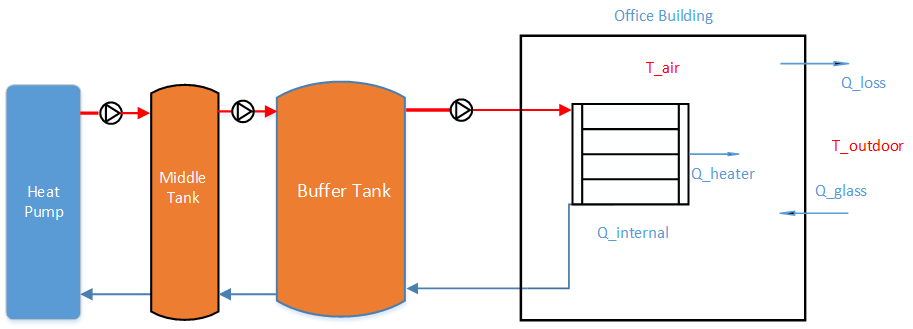
\includegraphics[width=1\columnwidth]{pictures/Office_diagram.png}
\caption[Short title]{Heating system layout for office building}
\label{fig:officeheatinglayout}\end{figure}

The room temperature can be calculated as:

\begin{equation}
C_{air}\frac{dT_{air}}{dt}=\frac{T_{outdoor}-T_{air}}{R_{air_{\_}outdoor}} + \frac{T_{wall}-T_{air}}{R_{air_{\_}wall}} + Q_{inst} + Q_{internal} + CF.Q_{solar}
\end{equation}

\begin{equation}
C_{wall}\frac{dT_{wall}}{dt}=\frac{T_{air}-T_{wall}}{R_{air_{\_}wall}} + (1-CF).Q_{solar}
\end{equation}

 \begin{itemize}
      \item CF: convectional factor.
      \item $Q_{inst}$: delivered heat from heating system (radiator) [W].
      \item $Q_{solar}$: heat from solar irradiation [W].
      \item $T_{air}$: indoor air temperature $^o$C.
      \item $T_{outdoor}$: outdoor temperature $^o$C.
      \item $T_{wall}$: wall temperature $^o$C.
      \item $R_{air_{\_}wall}$: walls surface resistance.
      \item $R_{air_{\_}outdoor}$: outdoor surface resistance.
      \item $C_{air}$: air capacity.
      \item $C_{wall}$: wall capacity.
    \end{itemize}
    

Total heat transfer of solar irradiation through the glass windows. 
\begin{equation}
Q_{solar}=g.\sum(A_{glass}.q_{solar})
\end{equation}

\begin{itemize}
    \item $q_{solar}$: solar radiation on the outdoor walls [$W/m^2$]. 
    \item g: g value of the glass (=ZTA in dutch) [0..1]
    \item A: glass surface [$m^2$].
\end{itemize}

\subsubsection{Apartment Building}

The system layout for an Apartment building is shown in Figure \ref{fig:ap_heatinglayout}. The configuration for space heating is similar with the office. The D.H.W is configured in parallel with space heating.

\begin{figure}[H]
\centering
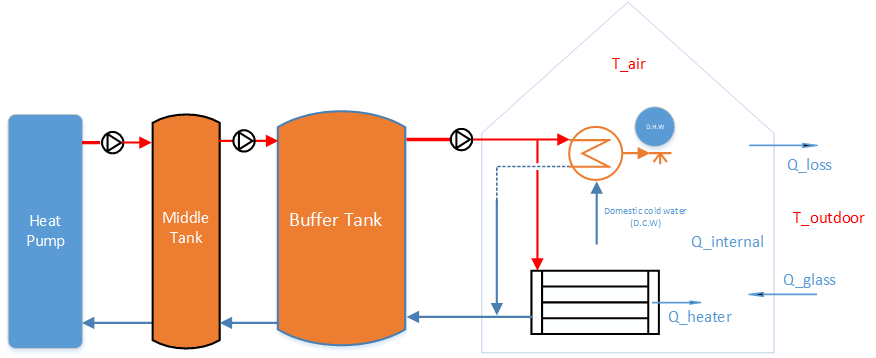
\includegraphics[width=1\columnwidth]{pictures/Apartment_diagram.png}
\caption[Short title]{Heating system layout for Apartment building.}
\label{fig:ap_heatinglayout}\end{figure}


The energy balance equation for space heating of an apartment is similar with office building (equation [1],[2]) where a single zone will be considered.

\[C_{air}\frac{dT_{air}}{dt}=\frac{T_{outdoor}-T_{air}}{R_{air_{\_}outdoor}} + \frac{T_{wall}-T_{air}}{R_{air_{\_}wall}} + Q_{inst} + Q_{internal} + CF.Q_{solar}\]

\[C_{wall}\frac{dT_{wall}}{dt}=\frac{T_{air}-T_{wall}}{R_{air_{\_}wall}} + (1-CF).Q_{solar}\]

The D.H.W consumption is base on D.H.W user profile and will be discussed in the next chapter.\\
The hot tap water temperature is calculated follow:

% \begin{equation}
%     c\rho V_{HE}\frac{dT_{tap}}{dt}= \alpha_{HE}2\pi r_{HE}\Delta x[T_{HE}(x+\Delta x,t)- T_{tap}] - c\rho F_{tap}(T_{tap} - T_{cold})
% \end{equation}

\begin{equation}
    c\rho V_{HE}\frac{dT_{tap}}{dt}= \alpha_{HE}2\pi r_{HE}\Delta x[T_{HE}(x+\Delta x,t)- T_{tap}] - Q_{D.H.W_{\_}profile}
\end{equation}

% \begin{align*}
% c\rho V_{HE}\frac{dT_{tap}}{dt}= \alpha_{HE}2\pi r_{HE}\Delta x[T_{HE}(x+\Delta x,t)- T_{tap}] - c\rho Ftap(T_{tap} - T_{water})\\

% c\rho V_{HE}\frac{dT_{tap}}{dt}= \alpha_{HE}2\pi r_{HE}\Delta x[T_{HE}(x+\Delta x,t)- T_{tap}] - P_{D.H.W_{\_}profile}
% \end{align*}

\begin{align}
    c\rho\pi r_{HE}^2\Delta x\frac{dT_{HE}(x+\Delta x)}{dt}=c\rho\Dot{m}[T_{HE}(x,t)-T_{HE}(x+\Delta x,t)]-\notag\\
    \alpha_{HE}2\pi r_{HE}\Delta x[T_{HE}(x+\Delta x,t)- T_{tap}]
\end{align}

% \begin{align*}
% c\rho\pi r_{HE}^2\Delta x\frac{dT_{HE}(x+\Delta x)}{dt}=c\rho\Dot{m}[T_{HE}(x,t)-T_{HE}(x+\Delta x,t)]-\\
% \newline \alpha_{HE}2\pi r_{HE}\Delta x[T_{HE}(x+\Delta x,t)- T_{tap}]
% \end{align*}
Where $T_{HE_{\_}in}$ = $T_{hot}$, $T_{HE_{\_}out}$ is the return water temperature from heat exchanger.

$T_{tap}$ is the hot tap water temperature $^oC$, $T_{HE}$ is the heat ex-changer temperature $^oC$, and $Q_{D.H.W_{\_}profile}$  is the hot tap water profile.



\subsection{Radiator equation}
Heat transfer from the radiators and the radiators outlet temperature is described as:
\begin{equation}
\frac{Q_{rad}}{dt}= Q_{in} -Q_{inst} - Q_{loss}
\end{equation}

With $Q_{inst}$ is the heat emission from a radiator. Its depends primarily on the temperature difference between the hot surface and the surrounding air(figure). The heat emission can be calculated: \cite{Radiators}

\begin{figure}[ht]
\centering
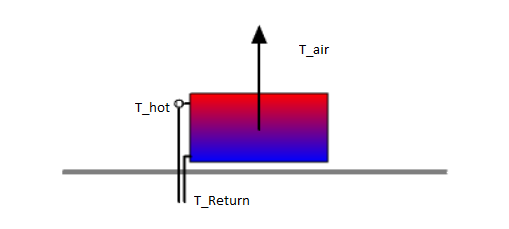
\includegraphics[width=1\columnwidth]{pictures/heat_emission_radiator.png}
\caption[Short title]{Heat emission from a radiator \cite{Radiators}.}
\label{fig:radiator}
\end{figure}

\begin{equation}
C_{rad}\frac{dT_{rad}}{dt} = \Dot{m}c\Delta T - Q_{50}\Big(\frac{LMTD}{49.32}\Big)^n
\end{equation}


\begin{align}
C_{rad}\frac{dT_{return}}{dt} = \Dot{m}c(T_{hot}-T_{return})\notag\\
- Q_{50}\Big(\frac{T_{hot}-T_{return}}{ln(T_{hot}-T_{air}) - ln(T_{return}-T_{air})}\frac{1}{49.32}\Big)^n
\end{align}


% \begin{align}
% c\rho r^2\Delta x\frac{dT_{rad1}}{dt} = \Dot{m}c(T_{hot}-T_{rad1}) \notag\\
% - U\frac{l}{\Delta x}A\frac{T_{hot}-T_{rad1}}{ln(T_{hot} -T_{air}) - ln(T_{rad1}-T_{air})}
% \end{align}

% \begin{align}
% c\rho r^2\Delta x\frac{dT_{return}}{dt} = \Dot{m}c(T_{rad1}-T_{return}) \notag\\
% - U\frac{l}{\Delta x}A\frac{T_{rad1}-T_{return}}{ln(T_{rad1} -T_{air}) - ln(T_{return}-T_{air})}
% \end{align}



\begin{itemize}
    \item LMTD: log mean Temperature Difference for the radiators.
    \item Crad: radiator constant.
    \item n: radiator exponent.
    \item $Q_{50}$: heat emission from radiator with temperature difference 50 $^oC$ [W]
    \item n: constant describing the type of radiator (1.33 for standard panel radiators, 1.3 - 1.6 for convectors). 
    \item $T_{rad}$: radiator temperature [$^oC$].
    \item $T_{hot}$: water temperature from buffer tank [$^oC$]. 
    \item $T_{return}$: water return temperature from radiator to the buffer tank [$^oC$].
    \item $T_{air}$: room temperature [$^oC$]. 
\end{itemize}
 Radiators are in general designed for middle panel temperature $70^oC$ - and surrounding air temperature $20^oC$ (difference $50^oC$)

\subsection{Water buffer}

In Figure \ref{fig:heatflow} to minimize the effect of water variation which can lead to the significant reduce in heat pump performance. The middle tank with a smaller size is placed in between Heat Pump and the main buffer.  

\begin{figure}[H]
\centering
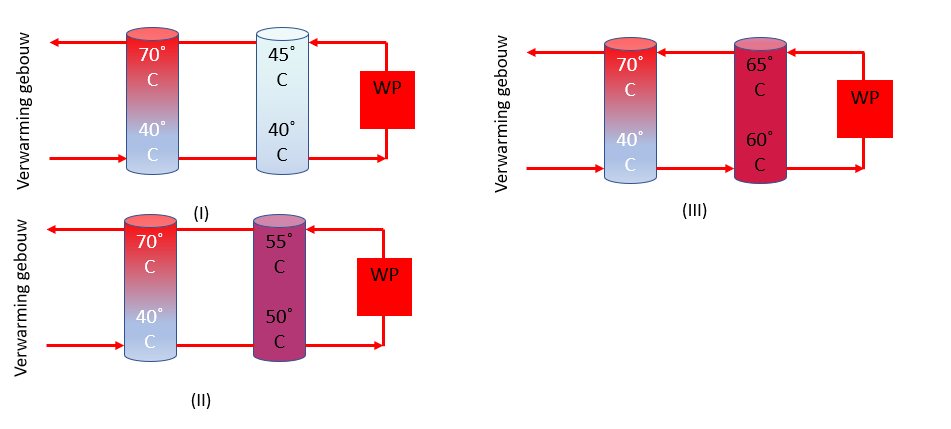
\includegraphics[width=1\columnwidth]{pictures/middle_tank.png}
\caption[Short title]{An illustration of heat flow.}
\label{fig:heatflow}
\end{figure}

The energy balance in the buffer tank can be determined:
% \begin{equation}
% \frac{dQ_{buffer}}{dt}= P_{in} -P_{out} - P_{loss}
% \end{equation}

\begin{equation}
c\rho V_{buffer}\frac{dT_{hot}}{dt}= c\rho \dot{m}(T_{mid_{\_}tank}-T_{hot}) - c\rho \dot{m}(T_{hot}-T_{return})
\end{equation}
\\
Where $V_{buffer}$ is the volume of the tank in $m^3$ 

$T_{mid_{\_}tank}$ is the temperature of the middle tank in $\degC$.

The energy balance in the middle tank:

% \begin{equation}
% \frac{dQ_{mid_{\_}tank}}{dt}= P_{in} -P_{out} - P_{loss}
% \end{equation}

% \begin{equation}
% c.\rho V_{mid_{\_}tank}\frac{dT_{mid_{\_}tank}}{dt}= c\rho \Dot{m}(T_{HP} - T_{mid_{\_}tank}) - c\rho \Dot{m}(T_{mid_{\_}tank} - T_{hot})
% \end{equation}

% or 

\begin{equation}
c.\rho V_{mid_{\_}tank}\frac{dT_{mid_{\_}tank}}{dt}= Q_{HP} - c\rho \Dot{m}(T_{mid_{\_}tank} - T_{hot})
\end{equation}

Where:
\begin{itemize}
    \item $V_{mid_{\_}tank}$ is the volume of the middle tank [$m^3$]
    \item $T_{mid_{\_}tank}$ water temperature inside the middle tank [$^oC$]. 
    \item $Q_{HP}$ Heat output from Heat Pump [W] 
    % \item $T_{HP}$ water temperature output from Heat Pump $^oC$.
\end{itemize}
 

\subsection{Heat Pump model from WP2}

